
\chapter{Instalación y despliegue de un \textit{cluster}}
En esta sección se cuenta el proceso para acondicionar las máquinas y así poder constituir un 
\textit{cluster} donde posteriormente instalar el software \textit{Hadoop}.
Previamente a la instalación de \textit{Hadoop} hay que configurar las máquinas con los requisitos 
necesarios e instalar distintos paquetes de \textit{software} para el correcto funcionamiento.\\
La instalación se ha realizado en 7 máquinas con las siguientes características:

\begin{table}[!htbp]
  \centering
  \begin{tabular}{|r|c|c|c|c|} % tabla
    \hline
    & \textcolor{Orange}{1 \textit{Manager}} & \textcolor{OliveGreen}{2 \textit{masters}} & \textcolor{BrickRed}{3 \textit{workers}} & \textcolor{blue}{1 \textit{gateway}} \\ \hline
    Sistema Operativo & CentOS 7 & CentOS 7 & CentOS 7 & CentOS 7 \\ \hline
    \textit{CPU} & 2 vcores & 2 vcores & 4 vcores & 2 vcores \\ \hline
    Memoria & $8gb$ & $4gb$ & $8gb$ & $4gb$ \\ \hline
    Disco duro & $40gb$ & $20gb$ & $80gb$ & $20gb$ \\ \hline
    \textit{GPU} & None & None & None & None \\ \hline
    \textit{Java} & $1.8.0\_101$ & $1.8.0\_101$ & $1.8.0\_101$ & $1.8.0\_101$ \\ \hline
    \textit{Python} & $2.7$ & $2.7$ & $2.7$ & $2.7$ \\ \hline
    Versión \textit{CDH} & $5$ & $5$ & $5$ & $5$ \\ \hline
  \end{tabular}
  \caption[\textit{Hardware} de las máquinas del \textit{cluster}]{Especificaciones de las máquinas}
  \label{cluster_machines_specification}
\end{table}

Con las máquinas disponibles lo primero que debemos hacer es elegir que máquina albergará cada rol dentro 
del \textit{cluster}, esto vendrá dado por los recursos disponibles de cada nodo y el uso que pretendamos hacer.
Hay que tener en cuenta que \textit{Hadoop} es escalable por lo que nuestro \textit{cluster} podrá 
ser ampliado en número de nodos según sea la demanda de recursos que necesitemos.\\
En nuestro caso, el reparto de roles queda así:

\begin{table}[!htbp]
  \centering Roles en el \textit{cluster} %texto cabecera
  \begin{tabular}{|r|c|c|c|c|c|c|c|} % tabla
    \hline
    & Master1 & Master2 & Worker1 & Worker2 & Worker3 & Gateway & Manager \\ \hline
    \textit{namenode} & \textcolor{OliveGreen}{\checkmark}  &  &  &  &  &  & \\ \hline
    \textit{secondary namenode} &  & \textcolor{OliveGreen}{\checkmark} &  &  &  &  & \\ \hline
    \textit{datanode} &  &  & \textcolor{BrickRed}{\checkmark} & \textcolor{BrickRed}{\checkmark} & \textcolor{BrickRed}{\checkmark} & & \\ \hline
    \textit{hdfs gateway} &  &  &  &  &  & \textcolor{Blue}{\checkmark} & \\ \hline
    \textit{resource manager} &  & \textcolor{OliveGreen}{\checkmark} &  &  &  &  & \\ \hline
    \textit{node manager} &  &  & \textcolor{BrickRed}{\checkmark} & \textcolor{BrickRed}{\checkmark} & \textcolor{BrickRed}{\checkmark} &  & \\ \hline
    \textit{job history server} & \textcolor{OliveGreen}{\checkmark} &  &  &  &  &  & \\ \hline
    \textit{yarn gateway} &  &  &  &  &  & \textcolor{Blue}{\checkmark} & \\ \hline
    
	\textit{cm server} & & & & & & & \textcolor{Orange}{\checkmark} \\ \hline
	\textit{cms database} & & & & & & & \textcolor{Orange}{\checkmark} \\ \hline
	\textit{cm service} & & & & & & & \textcolor{Orange}{\checkmark} \\ \hline
	\textit{cm agent} & \textcolor{Orange}{\checkmark} & \textcolor{Orange}{\checkmark} & \textcolor{Orange}{\checkmark} & \textcolor{Orange}{\checkmark} & \textcolor{Orange}{\checkmark} & \textcolor{Orange}{\checkmark} & \textcolor{Orange}{\checkmark} \\ \hline
    
  \end{tabular}
  \caption[Asignación de roles en el \textit{cluster}]{Asignación de roles entre máquinas}
  \label{asignacion_roles_cluster}
\end{table}

% Instalación de java y demás requisitos antes de instalar el software (cloudera repo, bases de datos, selinux...)
Como pasos previos a la instalación de los servicios del \textit{cluster}, se deben configurar 
ciertas propiedades del Sistema Operativo\index{Sistema Operativo} tales como parar el servicio \textit{iptables},
instalación de \href{https://es.wikipedia.org/wiki/Network_Time_Protocol}{NTP} para la sincronización de relojes, 
instalar el repositorio de \textit{Cloudera}...
Además de todo esto, debemos instalar Java ya que \textit{Hadoop} lo requiere para poder funcionar.

\clearpage

Todo este trabajo, si bien no es complicado, excede la longitud y los objetivos de este documento, por lo que he
omitido la inclusión de esta parte a la cual se puede acceder a través del siguiente link: 
\url{https://github.com/davidRetana/custom_centOS}
\newline

% Dar nombre a las máquinas
Antes de instalar el \textit{software}, tenemos que dar nombre a cada una de las máquinas que formaran el \textit{cluster}.
Esto se hace mapeando en el archivo \path{/etc/hosts} cada ip\index{IP} de la máquina con el nombre que la queramos dar.

\begin{lstlisting}[language=bash, numbers=none]
$ sudo vi /etc/hosts
\end{lstlisting}

\begin{figure}[!htpb]
  \centering
  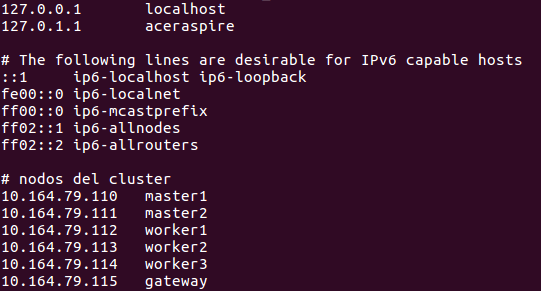
\includegraphics[width=\textwidth]{C:/Users/David/Desktop/TFG/TFGLatex/imagenes/etc_hosts.png}
  %\caption[archivo \path{/etc/hosts}]{resultado del archivo \path{/etc/hosts}}
  \label{etc_hosts}
\end{figure}

A continuación copiamos el archivo a cada máquina del \textit{cluster}:
\begin{lstlisting}[language=bash, numbers=none]
$ sudo scp /etc/hosts root@<ip_maquina_destino>:/etc/hosts
\end{lstlisting}

Para cada máquina del \textit{cluster} hacer:
\begin{lstlisting}[language=bash, numbers=none]
$ sudo hostname <nombre_de_la_maquina>
$ sudo vi /etc/sysconfig/network
\end{lstlisting}
En el archivo \path{/etc/sysconfig/network} cambiar HOSTNAME=<nombre máquina>
\newline

Para probar que los nodos se reconocen por su nombre lanzar el siguiente comando:
\begin{lstlisting}[language=bash, numbers=none]
$ ping <nombre_nodo_destino>
\end{lstlisting}
Si el nodo responde, lo hemos configurado bien.
\newline

% COMIENZO INSTALACION SOFTWARE
Para comenzar el despliegue del \textit{cluster}, instalaremos los dos servicios fundamentales para su 
correcto funcionamiento y sobre ellos se podrán añadir más servicios en un futuro. 
Sin embargo, este no es el objetivo del documento, y nos centraremos en instalar \textbf{\textit{HDFS}}, 
\textbf{\textit{YARN}} y posteriormente \textbf{\textit{Spark}}. 

\clearpage

\section{Instalación de \textit{HDFS} y \textit{YARN}}\label{sec:instalacion_hdfs_yarn}

En la máquina designada como \textit{Cloudera Manager} instalamos el servicio de \textit{cloudera-manager-server}

\begin{lstlisting}[language=bash, numbers=none]
$ sudo yum install cloudera-manager-server
\end{lstlisting}

Este comando nos instala el servicio en la máquina en cuestión. Una vez finalizado, se nos habrá creado el
directorio \path{/usr/share/cmf} dentro del cual tenemos que lanzar un \textit{script} que nos configura la base de 
datos que usa \textit{Cloudera Manager} por debajo

\begin{lstlisting}[language=bash, numbers=none]
$ sudo /usr/share/cmf/schema/scm-prepare-database.sh <base_de_datos> <nombre_db> \
  <usuario> <password>
\end{lstlisting}

A modo de ejemplo:

\begin{lstlisting}[language=bash, numbers=none]
$ sudo /usr/share/cmf/schema/scm-prepare-database.sh mysql cloudera root training
\end{lstlisting}

Si todo a funcionando correctamente, accedemos a \textit{mysql}\footnote{Sistema de gestión de base de datos relacional}\index{MySql} y vemos que se hayan creado correctamente las tablas

\begin{lstlisting}[language=bash, numbers=none]
$ mysql -uroot -ptraining

  mysql > show databases;
  mysql > exit;
\end{lstlisting}

Deberemos ver como las bases de datos \textit{amon} y \textit{rman} están creadas.\\
Finalmente arrancamos el servicio del \textit{cloudera-manager-server}

\begin{lstlisting}[language=bash, numbers=none]
$ sudo service cloudera-scm-server start
\end{lstlisting}

Este proceso tarda en terminar de ejecutarse pero una vez finalizado nos abrimos un navegador desde nuestro
portátil y escribimos en el campo de la url: \path{<ip_nodo_cloudera_manager>:7180}\\
A partir de ahora, será el asistente gráfico el que nos guíe a través del proceso de instalación del
\textit{cluster} en el resto de las máquinas. Para hacer el login inicial escribimos usuario:admin y 
password:admin, de esta manera ya estamos dentro del asistente gráfico.

\begin{figure}[!htpb]
  \centering
  \includegraphics[scale=0.5]{C:/Users/David/Desktop/TFG/TFGLatex/imagenes/capturas_cm/Captura1.JPG}
\end{figure}

Como se comento previamente, \textit{Cloudera Manager} es un software gratuito pero en su versión \textit{Cloudera Express},
sin embargo, tiene una versión de pago llamada \textit{Cloudera Enterprise} con funciones avanzadas para la gestión del
\textit{cluster} además de soporte. Esta opción esta disponible durante un mes a modo de prueba gratuita.
\newline

A lo largo de toda la instalación nos pedirá diversas opciones de configuración como por ejemplo el uso de
remesas de Cloudera, que son sencillamente abstracciones a nivel de repositorios de paquetes para que
podamos tener diferentes versiones de un mismo software sin que entren en conflicto y poder elegir que
versión usar en cada momento.
\newline

Como \textit{Cloudera Manager} necesita acceder a los nodos para desplegar paquetes de software e instalar agentes, necesita
acceder por \textit{SSH} a las máquinas por lo que nos pedirá la contraseña de los nodos del \textit{cluster}.
En este caso dicha contraseña deberá ser igual en todos los nodos.

\clearpage

\begin{figure}[!htpb]
  \centering
  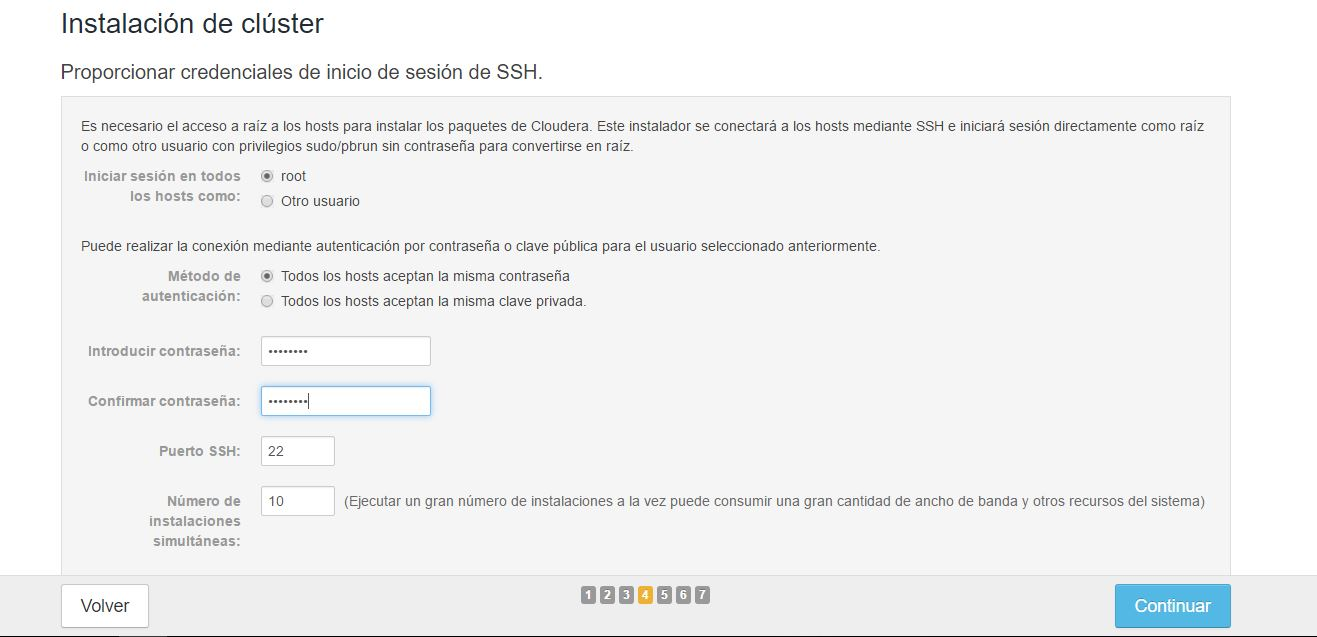
\includegraphics[width=\textwidth]{C:/Users/David/Desktop/TFG/TFGLatex/imagenes/capturas_cm/Captura8.JPG}
\end{figure}

A continuación se comenzará a descargar los paquetes de código y distribuirlos por las máquinas

\begin{figure}[!htpb]
  \centering
  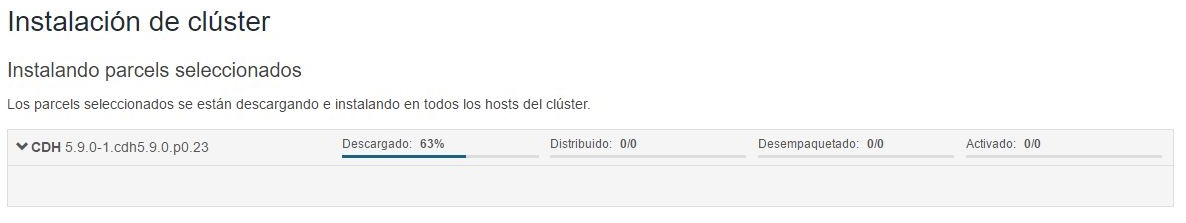
\includegraphics[width=\textwidth]{C:/Users/David/Desktop/TFG/TFGLatex/imagenes/capturas_cm/Captura11.JPG}
\end{figure}

Si todo funciona correctamente deberemos ver una pantalla como la siguiente:

\begin{figure}[!htpb]
  \centering
  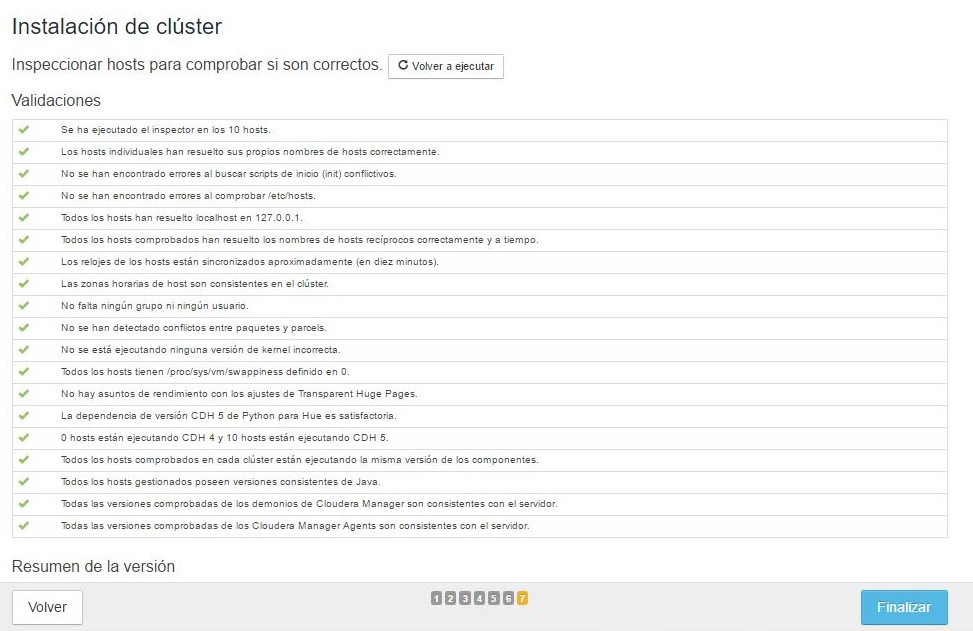
\includegraphics[width=\textwidth]{C:/Users/David/Desktop/TFG/TFGLatex/imagenes/capturas_cm/Captura16.JPG}
\end{figure}

Esta pantalla nos indica que todo ha salido correctamente. Comprueba entre otras cosas que los requisitos
mencionados al inicio del capítulo se cumplen y el despliegue del software ha sido satisfactorio.
\newline

Posteriormente, en la elección de los servicios a desplegar seleccionamos \textit{HDFS} y \textit{YARN} e
indicamos los nodos donde queremos que se instalen acorde a la \autoref{asignacion_roles_cluster}.\\
A continuación rellenamos las propiedades de los directorios donde los servicios de \textit{HDFS} y \textit{YARN}
dejarán los datos y habremos finalizado la instalación del \textit{cluster}.

\begin{figure}[!htpb]
  \centering
  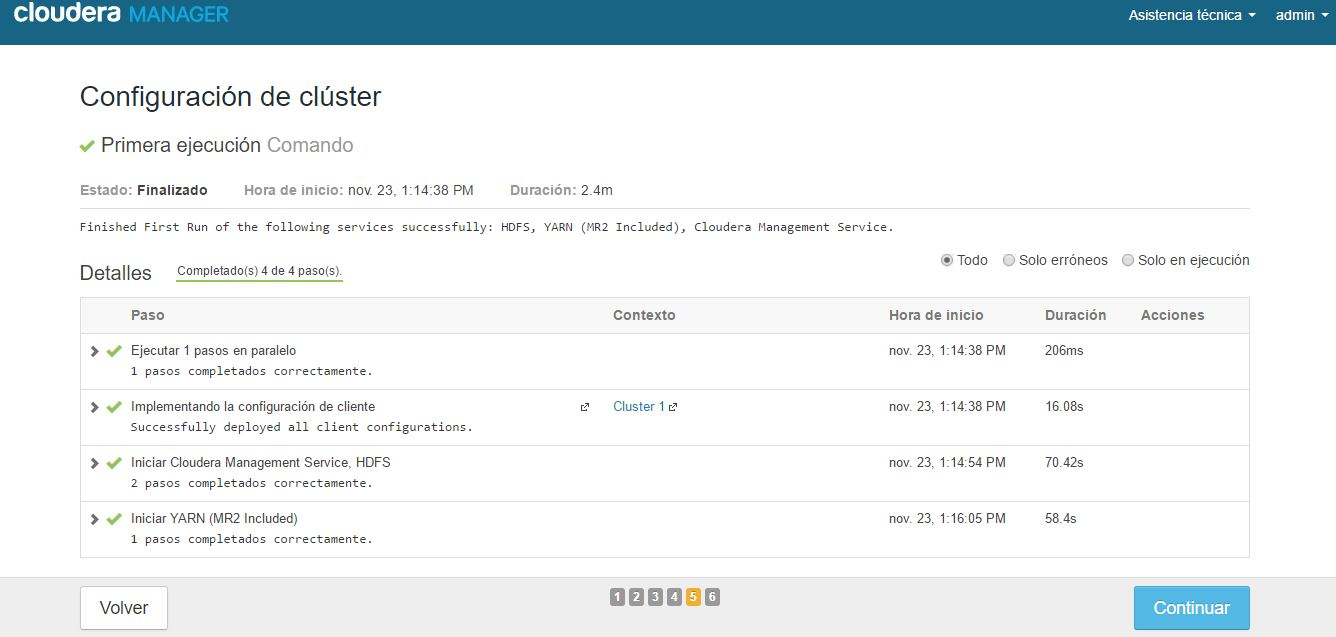
\includegraphics[width=\textwidth]{C:/Users/David/Desktop/TFG/TFGLatex/imagenes/capturas_cm/Captura23.JPG}
\end{figure}

Si todo fue satisfactoriamente, deberemos ser redirigidos a la página principal de administración de
\textit{Cloudera Manager}. Esta página será el punto de partida para cualquier configuración que queramos hacer
en el \textit{cluster}, así como añadir nuevos nodos, desplegar nuevos servicios, habilitar la alta
disponibilidad en el \textit{cluster} (HA\index{HA} por sus siglas en inglés 
\textit{High Availability}\footnote{Consiste en habilitar un segundo \textit{namenode} en el \textit{cluster} 
para evitar que un fallo en el nodo \textit{namenode} deje fuera de servicio al \textit{cluster} entero.})...\\
Además permite obtener métricas del uso de \textit{CPU}, I/O de red y de disco, etc.

\begin{figure}[!htpb]
  \centering
  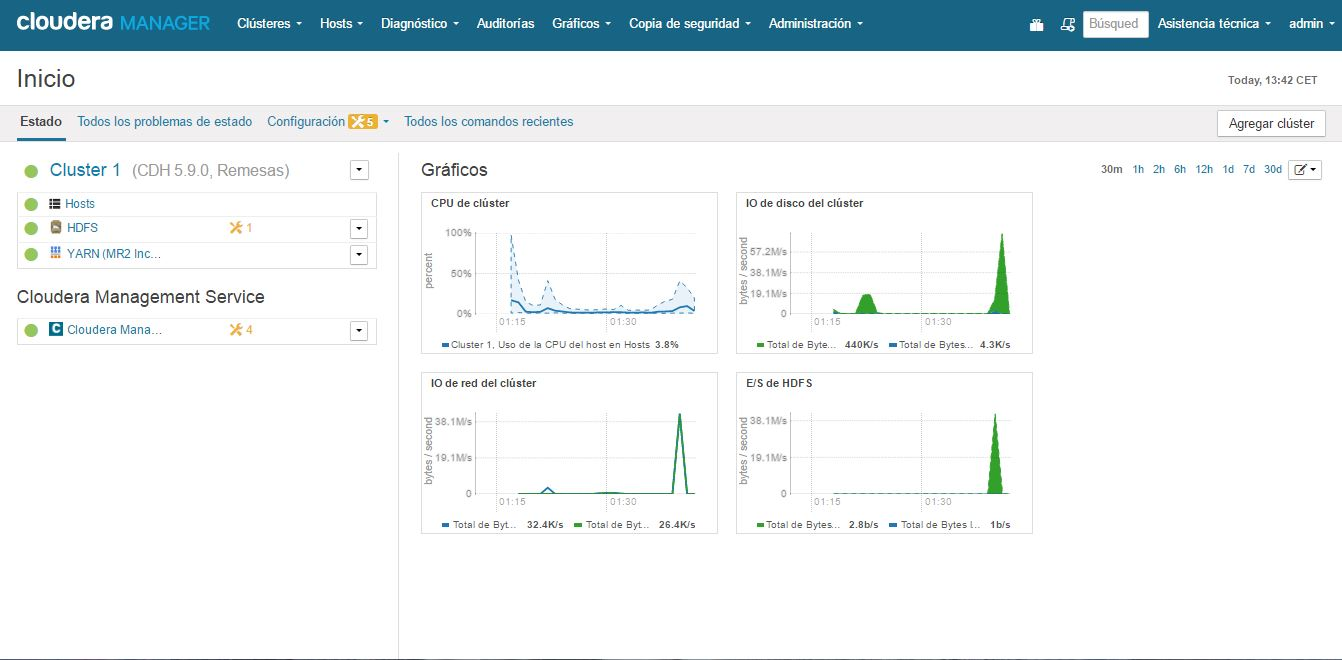
\includegraphics[width=\textwidth]{C:/Users/David/Desktop/TFG/TFGLatex/imagenes/capturas_cm/Captura26.JPG}
  \caption[Instantánea \textit{Cloudera Manager}]{Instantánea de la pagina principal de \textit{Cloudera Manager}}
\end{figure}

\subsection{Test del \textit{cluster} desplegado}\label{test_cluster_desplegado}
Para comprobar el correcto funcionamiento del \textit{cluster} instalado con \textit{Cloudera Manager}, vamos a subir
un archivo a \textit{HDFS}, veremos como se distribuye entre los nodos (en porciones de $128$ \textit{MB} por defecto) 
y luego ejecutaremos un trabajo \textit{MapReduce} que es el motor por defecto que utiliza \textit{YARN v2}.

\clearpage

Logeados en nuestra máquina \textit{gateway}, lo primero que debemos hacer es crearnos un directorio de trabajo
en \textit{HDFS} para nuestro usuario y darle permisos. Además vamos a crear un directorio temporal donde
todos los usuarios puedan escribir.

\begin{lstlisting}[language=bash, numbers=none]
$ # creacion de la home del usuario
$ sudo -u hdfs hdfs dfs -mkdir -p /user/<nombre_usuario>
$ sudo -u hdfs hdfs dfs -chown -R <nombre_usuario> /user/<nombre_usuario>
$ # creacion del directorio temporal
$ sudo -u hdfs hdfs dfs -mkdir -p /tmp
$ sudo -u hdfs hdfs dfs -chmod -R 1777 /tmp
\end{lstlisting}

Hecho esto, lanzamos el comando para subir un archivo que esta en local a \textit{HDFS} y luego comprobamos
que realmente se ha subido:

\begin{lstlisting}[language=bash, numbers=none]
$ hdfs dfs -put <path_archivo_local> <path_en_hdfs>
$ hdfs dfs -ls
\end{lstlisting}

Si todo ha funcionado correctamente, abrimos un navegador y escribimos \path{<ip_namenode>:50070}

\begin{figure}[!htpb]
  \centering
  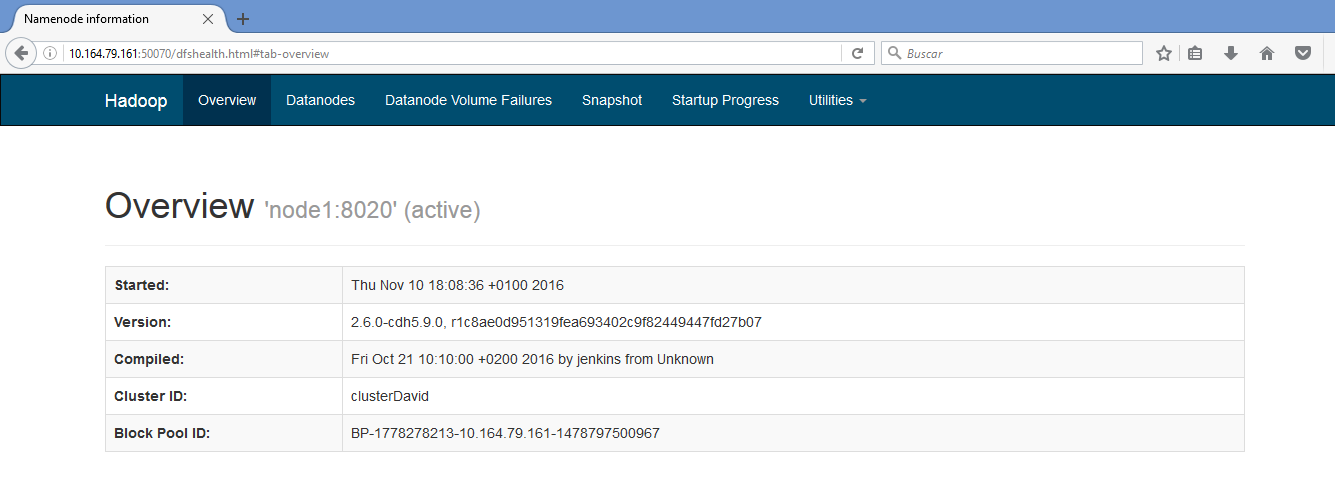
\includegraphics[width=\textwidth]{C:/Users/David/Desktop/TFG/TFGLatex/imagenes/capturas_creacion_cluster/1.png}
  \caption[\textit{Overview web namenode}]{\textit{Overview} del servicio web del \textit{namenode}}
\end{figure}

Si nos vamos a la pestaña de \textit{Datanodes} veremos los nodos trabajadores que tenemos activos y su 
capacidad de almacenamiento entre otras cosas.

\begin{figure}[!htpb]
  \centering
  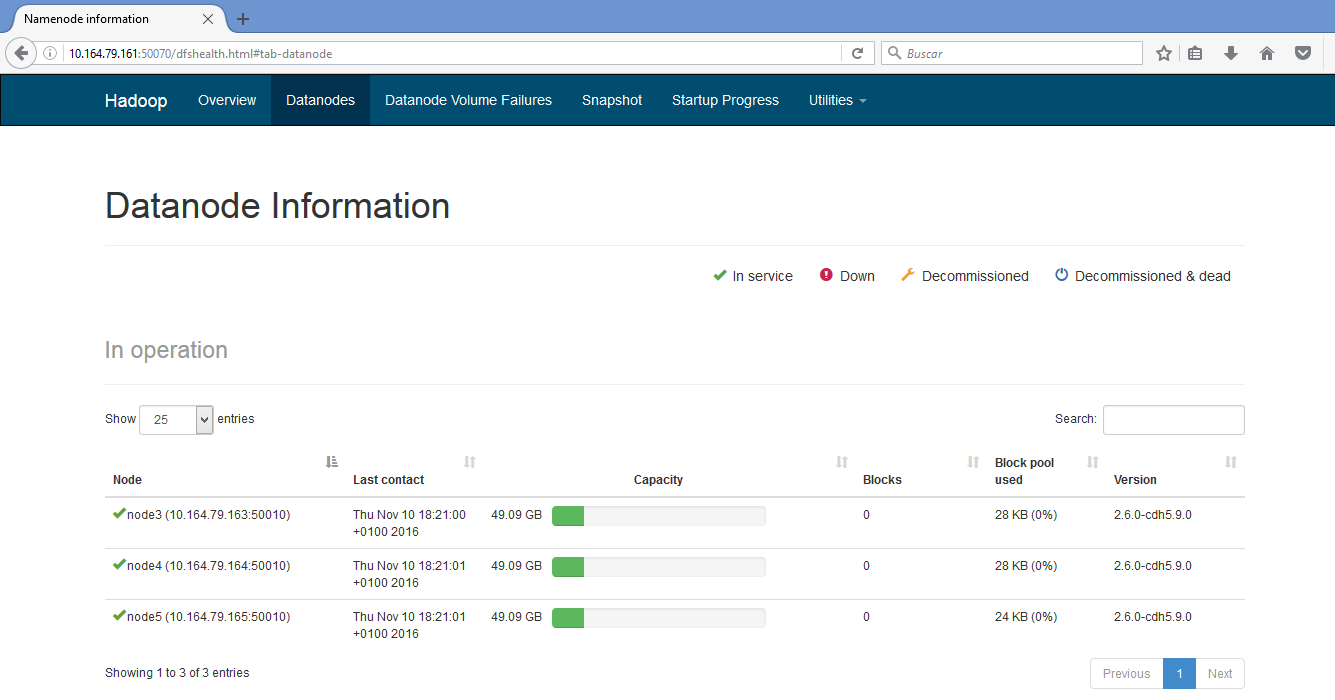
\includegraphics[width=\textwidth]{C:/Users/David/Desktop/TFG/TFGLatex/imagenes/capturas_creacion_cluster/5.png}
  \caption[Información web \textit{Datanode}]{Información de los \textit{datanodes}}
\end{figure}

\clearpage

Para testear \textit{YARN}, vamos a lanzar un trabajo \textit{MapReduce} en dos fases, una primera donde
solo se ejecute la fase \textit{map} y luego otra donde solo se ejecute la fase \textit{reduce}.

\begin{lstlisting}[language=bash, numbers=none]
$ hadoop jar /usr/lib/hadoop-mapreduce/hadoop-mapreduce-examples-2.6.0-cdh5.9.0.jar \
   teragen 10000 output_prueba_teragen
\end{lstlisting}

Veremos una salida parecida a esta:

\begin{figure}[!htpb]
  \centering
  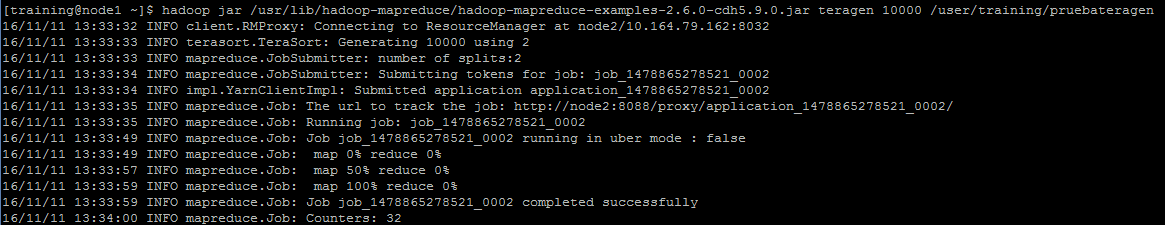
\includegraphics[width=\textwidth]{C:/Users/David/Desktop/TFG/TFGLatex/imagenes/capturas_creacion_cluster/12.png}
\end{figure}

Ahora ejecutaremos la fase reduce donde recibirá como entrada la salida del trabajo anterior

\begin{lstlisting}[language=bash, numbers=none]
$ hadoop jar /usr/lib/hadoop-mapreduce/hadoop-mapreduce-examples-2.6.0-cdh5.9.0.jar \
   terasort output_prueba_teragen output_prueba_terasort
\end{lstlisting}

Donde nuevamente veremos una salida parecida a esta:

\begin{figure}[!htpb]
  \centering
  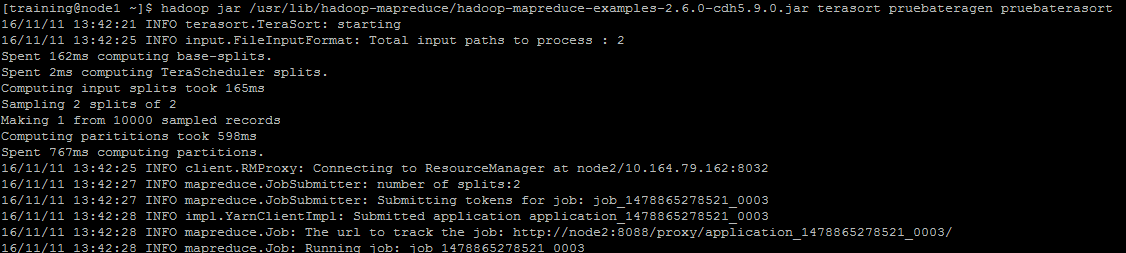
\includegraphics[width=\textwidth]{C:/Users/David/Desktop/TFG/TFGLatex/imagenes/capturas_creacion_cluster/15.png}
\end{figure}

Si nos vamos a un navegador y escribimos \path{<ip_resourcemanager>:8088}, veremos de una manera gráfica
los trabajos que se están ejecutando en nuestro \textit{cluster}, el historial de trabajos subidos, la
memoria utilizada, los contenedores asignados...\\
Llegados a este punto, ya tendremos un \textit{cluster} totalmente operativo con los servicios de
\textit{HDFS} Y \textit{YARN} instalados correctamente.

\begin{figure}[!htpb]
  \centering
  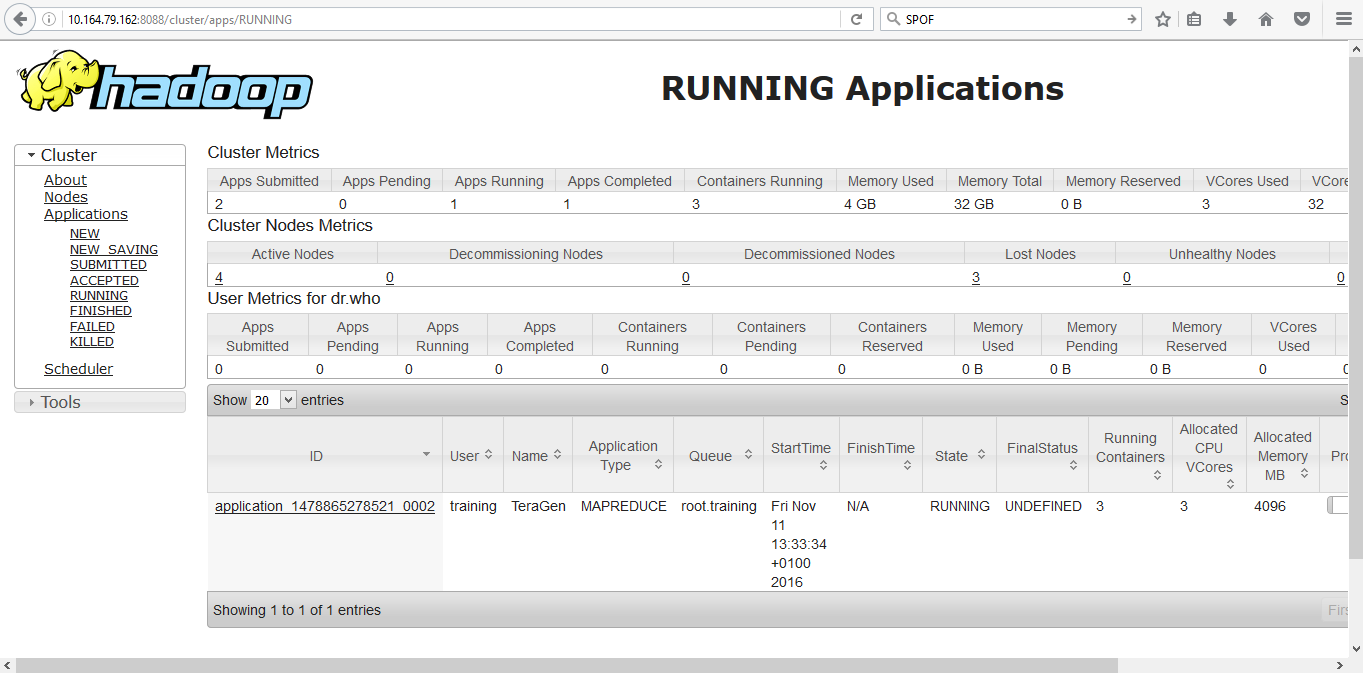
\includegraphics[width=\textwidth]{C:/Users/David/Desktop/TFG/TFGLatex/imagenes/capturas_creacion_cluster/11.png}
  \caption[Web del servicio \textit{Resource Manager}]{Web del servicio \textit{resource manager}}
\end{figure}

\clearpage

\section{Instalación de \textit{Apache Spark}}\label{sec:instalacion_spark}
             
\begin{wrapfigure}[]{l}{0.5\textwidth}
  \centering
  \includegraphics[width=0.5\textwidth]{C:/Users/David/Desktop/TFG/TFGLatex/imagenes/capturas_spark/Captura1.JPG}
\end{wrapfigure}

Para la instalación de \textit{Apache Spark}, desde la página principal de administración de \textit{Cloudera Manager}
seleccionamos la pestaña 'Agregar un servicio' en el desplegable de \textit{cluster}.
En esta pestaña están disponible todos los servicios soportados por Cloudera y que por lo tanto son compatibles
con nuestro \textit{cluster}.\\
Nota: Ya se encuentra disponible la version $2.0$ de \textit{Spark}, pero su
instalación es algo diferente ya que debe hacerse desde las \textit{parcels} de Cloudera. Esto es así porque
las versiones $2.x.x$ son incompatibles con las versiones $1.x.x$
\newline

La opción de \textit{Spark} que cogeremos será aquella que utilice \textit{YARN} como gestor de recursos del
\textit{cluster}.
Notese que la opción \textit{Spark} (\textit{Standalone}\footnote{\textit{Standalone} es un modo de despliegue
autónomo, no requiere de ningún gestor de recursos del \textit{cluster}.}
\index{Standalone}) también está disponible.

\begin{figure}[!htpb]
  \centering
  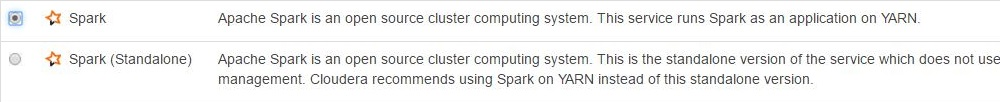
\includegraphics[width=\textwidth]{C:/Users/David/Desktop/TFG/TFGLatex/imagenes/capturas_spark/Captura2.JPG}
\end{figure}

Una vez hecho esto, elegimos la máquina que hemos etiquetado como \textit{gateway} para desplegar el servicio
de \textit{Spark} ya que será desde esta máquina donde subiremos nuestros trabajos 
\textit{spark-submit}\index{Spark-submit} o \textit{pyspark}\index{Pyspark} al \textit{cluster}.
Después de todo este proceso de instalación, nuestra pagina principal de \textit{Cloudera Manager} debería lucir los 
3 servicios que hemos instalado.

\begin{figure}[!htpb]
  \centering
  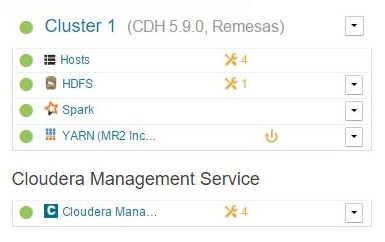
\includegraphics[width=0.6\textwidth]{C:/Users/David/Desktop/TFG/TFGLatex/imagenes/capturas_spark/Captura5.JPG}
\end{figure}

Lo ultimo que nos queda por hacer es reiniciar el servicio de \textit{YARN} para que hagan efecto
los cambios que hemos realizado en el \textit{cluster}.

\begin{figure}[!htpb]
  \centering
  
\includegraphics[width=0.6\textwidth]{C:/Users/David/Desktop/TFG/TFGLatex/imagenes/capturas_spark/Captura5_paint.JPG}
\end{figure}

Seguimos el asistente de reinicio y habremos terminado la instalación de \textit{Spark}.
\newline

Para comprobar su correcto funcionamiento iniciamos un intérprete \textit{pyspark} desde la máquina \textit{gateway}
\begin{lstlisting}[language=bash, numbers=none]
$ pyspark --master local[*]
\end{lstlisting}

\clearpage

\begin{figure}[!htpb]
  \centering
  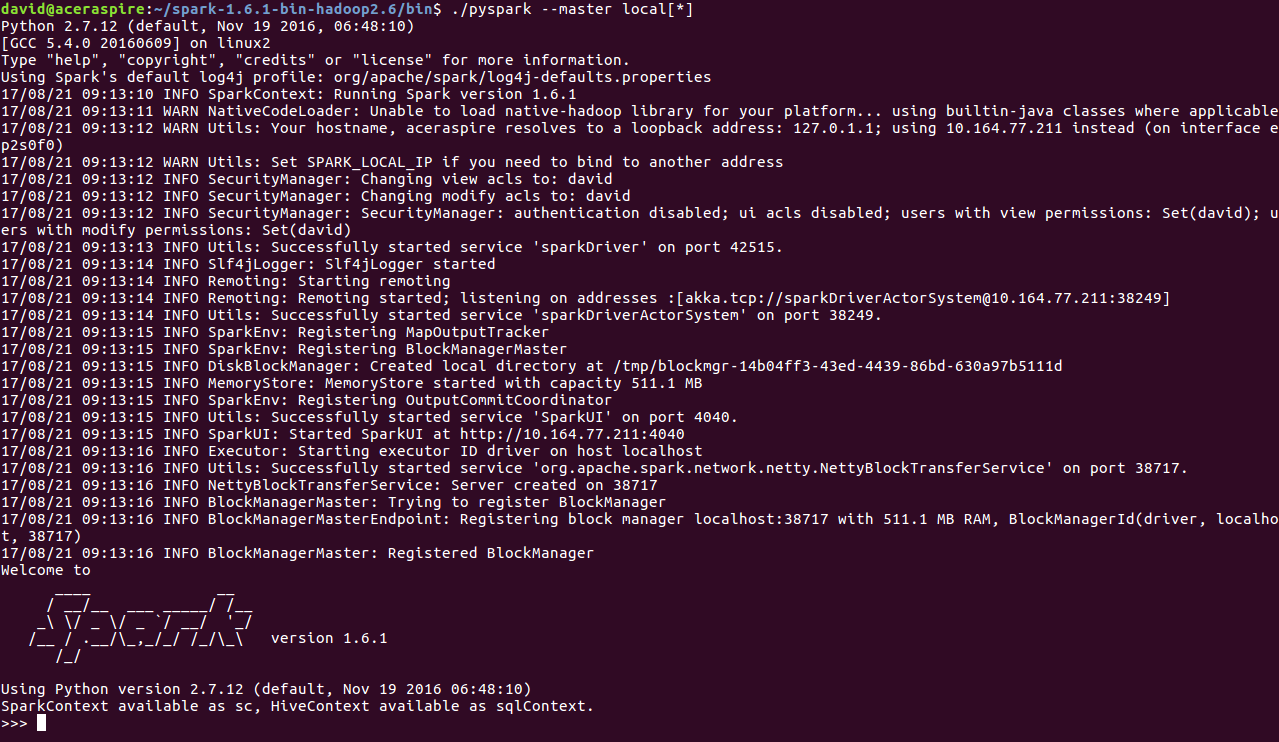
\includegraphics[width=\textwidth]{C:/Users/David/Desktop/TFG/TFGLatex/imagenes/pyspark_shell.png}
  \caption[\textit{PySpark shell}]{\textit{PySpark shell}}
  \label{pyspark_shell}
\end{figure}

En esta terminal tendremos creadas por defecto las variables \textit{sc} (\textit{Spark Context}\index{Spark Context})
y \textit{sqlContext}\index{SQLContext}. La primera es el punto de partida para una aplicación \textit{Spark}, mientras
que la segunda habilita características de SQL para el tratamiento de datos.\\
Si queremos comprobar que todo funciona correctamente podemos ejecutar las siguientes ordenes de \textit{pyspark}:

\begin{lstlisting}[language=bash, numbers=none]
 >>> rdd = sc.parallelize(range(100))
 >>> rdd.count()
\end{lstlisting}

Con estas ordenes lo que estamos diciendo es que se paralelice la lista de enteros que va desde el 0 hasta el 99,
distribuyéndola entre los nodos, y luego desencadenando una acción que es el contar el número de elementos.
Si la orden se completa, hemos instalado correctamente \textit{Spark} en nuestro \textit{cluster}.

\section*{Conclusión del despliegue}

Esto concluye el despliegue de un \textit{cluster} realizado con \textit{Cloudera Manager}, donde hemos instalado los
servicios básicos de \textit{Hadoop} y además el motor de procesamiento \textit{Spark}.\\
En el siguiente capítulo se comentará las diferencias entre los distintos enfoques de procesamiento y se
explica en que consisten los \textit{frameworks} de \textit{MapReduce} y \textit{Spark}.
En la \autoref{part:analisis_datos} (\nameref{part:analisis_datos}) se utiliza el \textit{cluster} construido 
en esta sección para entrenar los modelos de \textit{machine learning} y reducir sus tiempos de ejecución.

\clearpage
